% TODO units

Figure \ref{fig:system_design} illustrates our general system design approach
that simulates the ecovisor infrastructure and integrates it into the Mosaik
co-simulation environment while enabling SIL capabilities. The present design
can be categorized into two distinct parts, the simulation of the ecovisor, and
its interface to external applications, which are elaborated on in the
following.

\begin{figure}
    \centering
    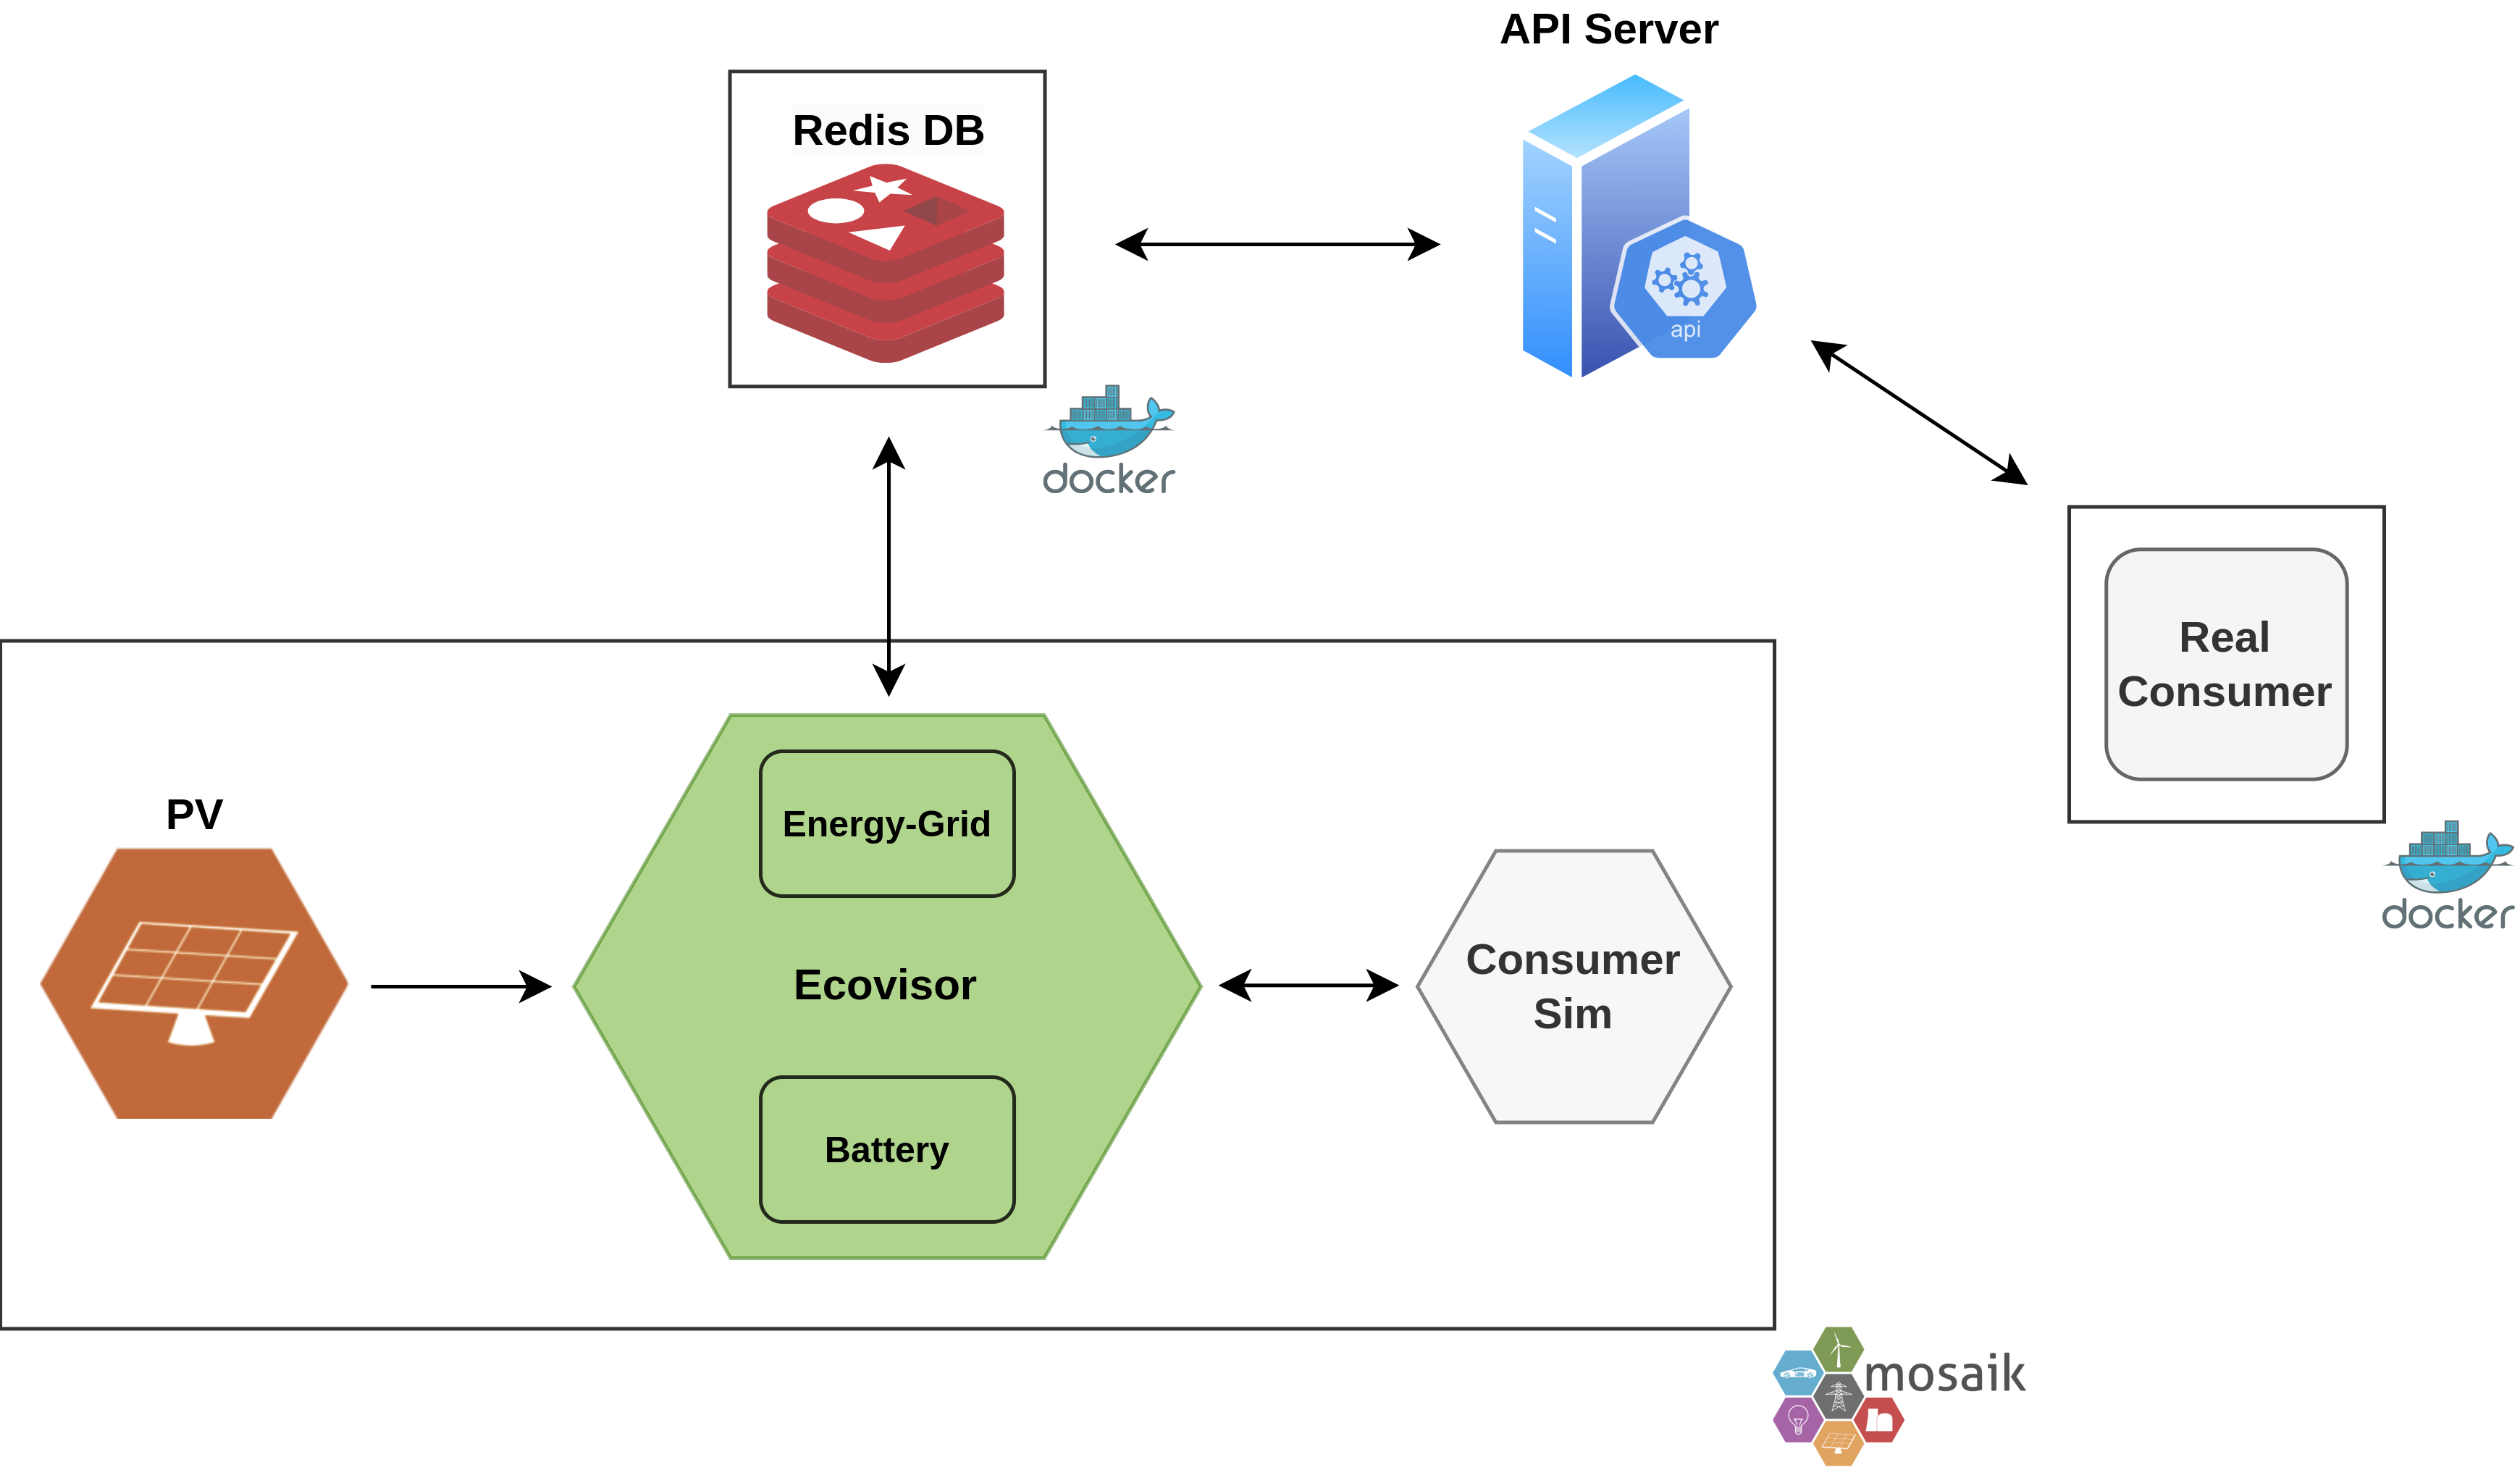
\includegraphics[width=\linewidth]{figures/system_design}
    \caption{
        General System Design: The ecovisor infrastructure is simulated and
        integrated into the Mosaik co-simulation environment. SIL capabilities
        are enabled via an API Server and a Redis database, connecting the
        simulation environment and real applications in real-time.
    }
    \label{fig:system_design}
\end{figure}

\subsection{Simulation of the Ecovisor}

\begin{figure}
    \removelatexerror
    \begin{algorithm}[H]
        \caption{Virtual Energy System Simulation}
        \label{alg:virtual_energy_system_simulation}
        $rest \gets consumption - solar$\;
        \eIf{$rest \leq 0$} {
            $b\_discharge\_rate \gets 0$\;
        }{
            $b\_discharge\_rate \gets \text{min}($\;
            \Indp
                $b\_max\_discharge,$\;
                $b\_charge\_level \cdot 3600,$\;
                $rest$\;
            \Indm
            $)$\;
            $rest \gets rest - b\_discharge\_rate$\;
        }
        $grid\_power \gets b\_charge\_rate + rest$\;
        $b.delta \gets b\_charge\_rate - b\_discharge\_rate$\;
        $b.step()$\;
        $b\_charge\_level \gets b.charge$\;
        $total\_carbon \gets grid\_carbon \cdot grid\_power$\;
        \vspace{3mm}
    \end{algorithm}
\end{figure}

\subsection{Interface to External Applications}
%ToDo: Second itteration on writing

For connecting the Ecovisor-Model to a real workload, we had to expose the API described in \cite{souza2023}. We have tried to implement it as it would probably be implemented in a real cloud environment. %source?
To achive that, we implemented the API of the Ecoviser with a RedisDB as value store between the ecovisor and the api-server. This also ensures atomiticity on the writes of the values. %sourec

The API integration itself consists of three parts, the API-Server, the RedisDB and the Ecovisor-Redis-Interface which are described in the following sections.
%Picture API
%\begin{figure}
%    \centering
%    \includegraphics[width=\linewidth]{}
%    \caption{Ecovisor API}
%    \label{fig:ecovisor_api}
%\end{figure}



\subsubsection{API-Server}
The API Server exposes the Ecoviser-API to the "Workloads". It is implemented with the FastAPI Framework and Utilizes Uviorn to handel multiple clients accessing the API.
The Module is started as aan independent thread. In earlyer versions we tried to implement it inside of the ecovisor model, but due to the way uvicorn starts the API-Server,
it would stops the execution of the simulation until the API-Server is stopped and so we decided to design it as a standalone module. This als enables the API-Server to be scaled indipendetn from
the Ecovisor-Model and the RedisDB. This may be helpful in bigger simulations with distributed infrastructur. 


\subsubsection{RedisDB}
The RedisDB is used to interchange the values provided by eiterh ecovisor or the workload application. The database itself is a fast in memory key value store, wich is started as a docker container via the docker python libary %quelle pyton lib
to keep manual managment of the simulation to a minimum.

Since the values are updated in one write atomicity is ensured, but due to the dataflow described in \ref{subsec:dataflow}
atomicity isnot requierd to keep the values consistent.

In general the Database can be exchanged with any other database by adapting the Ecovisor-Redis-Interface in the Ecovisor model. This can be useful when simulation should be integrated 
in a production grade cloud environment like kubernetes or openstack.

%values picture
%\begin{figure}
%    \centering
%    \includegraphics[width=\linewidth]{}
%    \caption{Datastructur of exchanged Data}
%    \label{fig:ecovisor_api}
%\end{figure}

\subsubsection{Ecovisor-Redis-Interface}
The interface from the ecovisor towards the redisdb is implemented within the ecovisor model. To simplify the usage, the redis python libary %source
is used. The ecovisor model implements two methods, the get_redis_updates() and the send_redis_updates %methoden mit code abgleicehn und formatieren

The get_redis_update method gets the values (...) as show in (ref) from the RedisDB %insert valzes and reference to the 
and writes it to the ecovisor model variables to make them usable for the ecovisor model.

the send_redis_updates() method publishes the updated values from the other part of the simulation which are accessible by the ecoviser shwon in (ref) model to the redisdb to make it
usable by the workload application. %raus wegen dopplung?

In each step the ecovisor model first gets the updates from the RedisDB, processes the data and then sends the updated data to the RedisDB, to make it
acessible to the workload application.  

%code?
\subsubsection{Dataflow}\label{subsec:dataflow}
%Picture Data-Flow (Values set by Ecovisor, Values set by Workload)
%\begin{figure}
%    \centering
%    \includegraphics[width=\linewidth]{}
%    \caption{Dataflow betwen Ecovisor and API Server}
%    \label{fig:ecovisor_api}
%\end{figure}

The Values/Data shown in (ref) is exchanged between the ecovisor model and the API server via the RedisDB. There are two main streams of the dataexchange.
First from the ecovisor model to the API-Server and second from the API-Server to the ecovisor model. There are no values which are used in both streams, which makes things
easier in terms of consistency and parallel access. 

As stated before, the data is updated in each simulation step. (ref) 
In the downstream, from the ecovisor to the API-Server the values (...) are updated and can be consumed by the workload applications
and in the upstream, from the api-server to the ecovisor model, the values (...) are updated and used by the ecovisor model to calculate (...) %abgleich mit code
%referenz bild einbinden

